\documentclass{article}

% Lenguaje y Fuente
\usepackage[spanish]{babel}
\usepackage[utf8x]{inputenc}
\usepackage[T1]{fontenc}
\usepackage[top=1in, bottom=1.25in, left=1.1 in, right=1.1 in]{geometry}
\usepackage{graphicx}
\usepackage{ragged2e}
\usepackage[usenames]{color}
\usepackage{multicol}

% Portada

\title{\textbf{Reporte de la Actividad 4}\\ Introducción a la Biblioteca de Visualización Matplotlib}
\author{Luis Fernando Duarte Gonzalí \\ Universidad de Sonora \\ Física Computacional}
\date{Febrero del 2019}
\begin{document}
\maketitle

% Contenido del Reporte

\section{Introducción}
\noindent En el siguiente documento se abordará el tema de la biblioteca Matplotlib de Python como introducción, se mostrarán en gráficas los datos obtenidos en el reporte anterior. Seguiremos trabajando con el documento de \textit{Leon.txt}, ahora desde el punto de visualización.

El archivo que se analizó fue descargado de la página del servicio meteorológico de la columna de medias y extremas diarias.

\subsection{Matplotlib}
\noindent Matplotlib es una librería de en Python que produce gráficas en diferentes ambientes interactivos. En él puedes dibujar diferentes tipos de gráficos, como las de evolución, de dispersión, de barras, etc. Es mayormente usado en python y R para visualizar gráficos y permitir la exploración de datos.

\section{Análisis de Datos}

\noindent Para comenzar, necesitamos abrir \textsc{Jupyter Lab} desde Anaconda Prompt, abriendo la carpeta creada previamente con el nombre de \textit{Actividad3}.
Una vez abierto, en python, primero se importaron las bibliotecas Pandas, Numerical Python y Matplot para generar las gráficas.

\begin{center}
    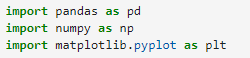
\includegraphics[scale = 1]{Librerias.png}
\end{center}

\noindent Se leyó el archivo de texto, definiéndole una variable, también se saltaron los renglones innecesarios que fueron 4 para después estructurar los datos de mejor manera con \textit{DataFrame}.

\begin{center}
    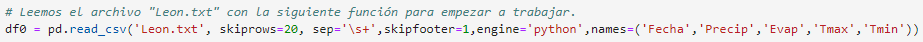
\includegraphics[scale = .65]{read.png}
    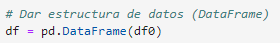
\includegraphics[scale = .8]{DataFrame.png}
\end{center}
\clearpage

Para que python pudiera leer los archivos nulos, fue necesario reemplazar la palabra \textit{Nulo} por NaN. Además de cambiar los tipos de datos para poder trabajar con ellos.
\begin{center}
    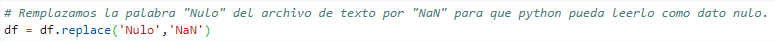
\includegraphics[scale = .74]{NaN.png}
    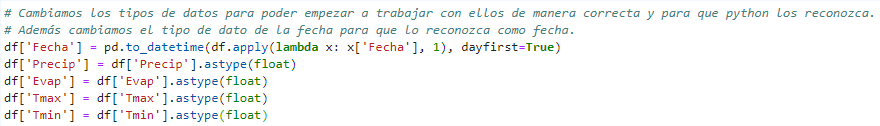
\includegraphics[scale = 0.65]{Float.png}
\end{center}

\section{Resultados}
\noindent En esta sección sólo se mostrarán las gráficas requeridas para el análisis básico de datos a manera de práctica e introducción a Matplotlib.

\subsection{Gráfica de Barras}
\subsubsection{Código para visualizar el promedio de la precipitación por mes}
\begin{center}
    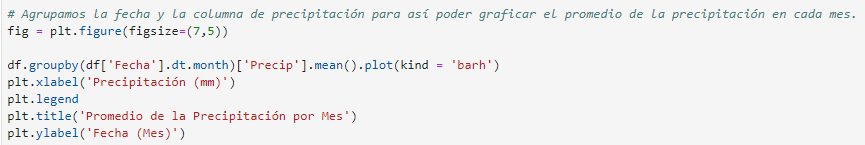
\includegraphics[scale = 0.65]{CPrecip.png}
\end{center}

La siguiente gráfica nos muestra la precipitación mensual acumulada promedio de la colección de datos de la estación que se esté analizando.

\begin{center}
    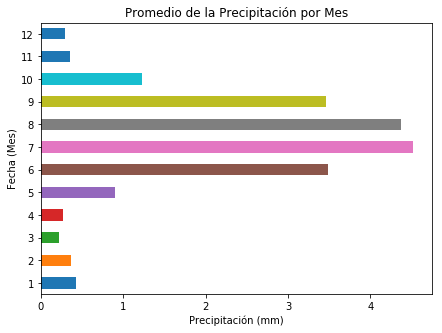
\includegraphics[scale = 0.75]{Precip.png}
\end{center}
\subsubsection{Código para visualizar la precipitación acumulada cada año}
\begin{center}
    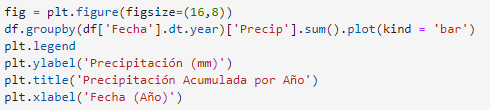
\includegraphics[scale = 0.9]{CPrecipY.png}
\end{center}
La gráfica que observamos a continuación nos de precipitación acumulada para cada año de la mima colección. Por eso en el código utilizamos la función \textit{.sum()}.
\begin{center}
    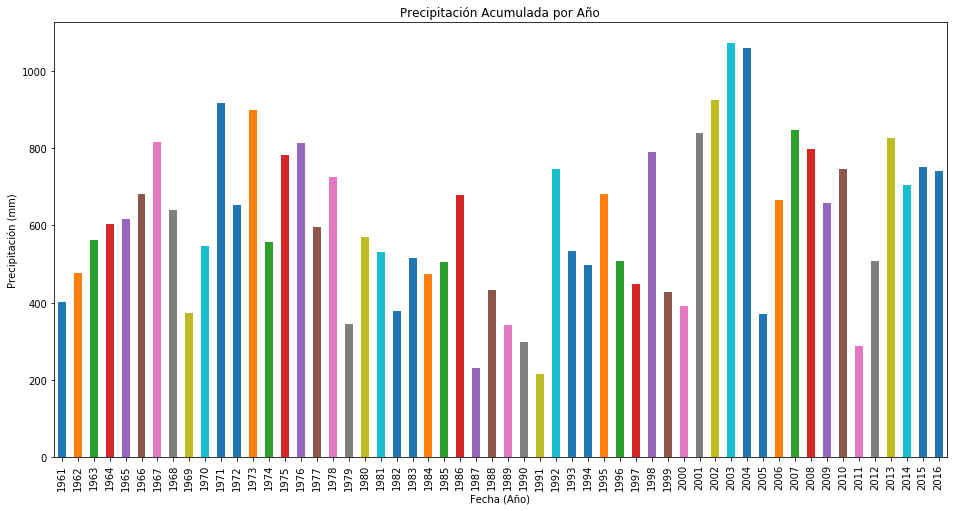
\includegraphics[scale = 0.474]{PrecipY.png}
\end{center}

\subsection{Gráfica de la Evolución de Temperatura}
\subsubsection{Código para visualizar la evolución temporal de la Temperatura}
\begin{center}
    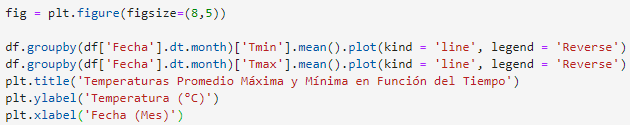
\includegraphics[scale = 0.9]{CTemp.png}
\end{center}

\clearpage
Lo que nos generó la siguiente gráfica, donde vemos la temperatura mínima y máxima como función del tiempo:
\begin{center}
    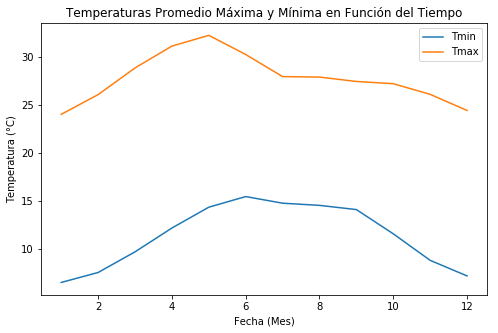
\includegraphics[scale = 0.70]{Temp.png}
\end{center}
\subsection{Gráfica de Cajas}

\subsubsection{Código para visualizar la temperatura promedio mensual}
\noindent Primero se crearon nuevas columnas que contuvieran sólo el mes y sólo el año para poder graficar los diagramas de caja en una sola gráfica.
\begin{center}
    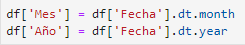
\includegraphics[scale = 0.9]{MY.png}
\end{center}
Después se escribieron los códigos para generar las gráficas de cajas como se muestran en las siguientes figuras:
\begin{center}
    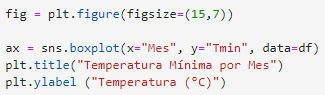
\includegraphics[scale = 0.9]{CTminBoxM.png}
    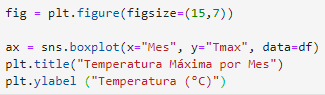
\includegraphics[scale = 0.9]{CTmaxBoxM.png}
\end{center}
\clearpage
Esos códigos nos permitieron visualizar las siguientes gráficas para la Temperatura Máxima y Mínima por Meses.
\begin{center}
    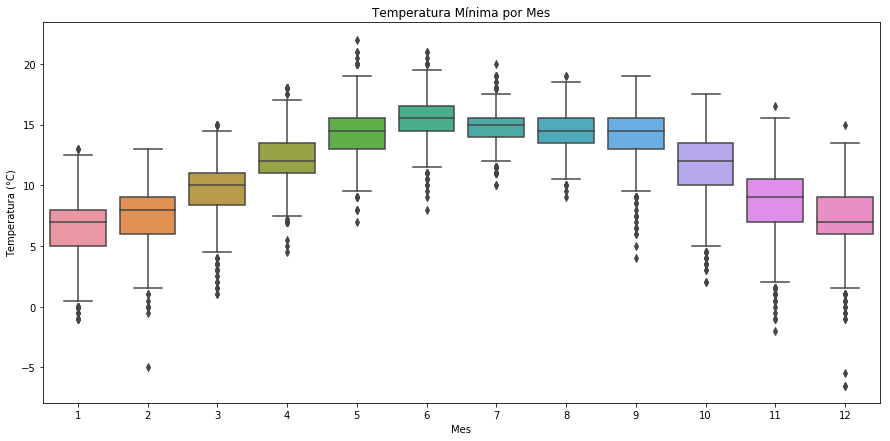
\includegraphics[scale = 0.45]{TminBoxM.png}
    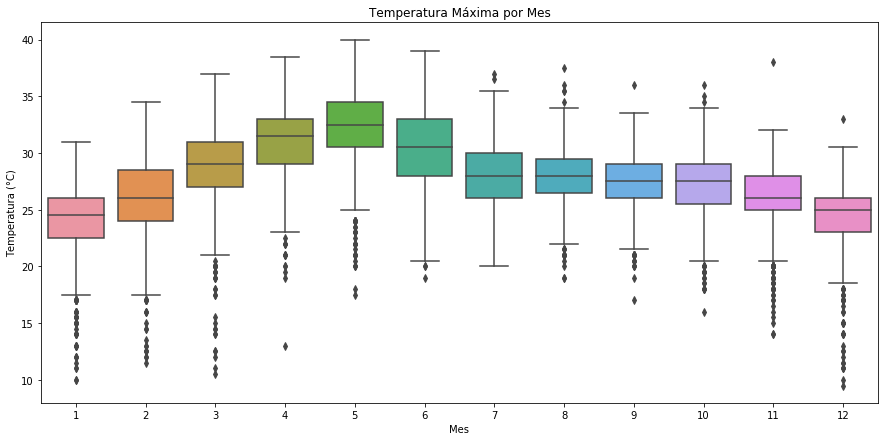
\includegraphics[scale = 0.45]{TmaxBoxM.png}
\end{center}
\subsubsection{Código para visualizar la temperatura promedio anual}
\noindent Se escribieron los códigos para generar las gráficas de cajas para la temperatura mínima y máxima anual como se muestran en las siguientes figuras:
\begin{center}
    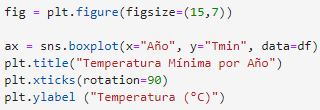
\includegraphics[scale = 0.9]{CTminBoxY.png}
    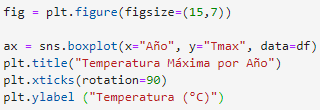
\includegraphics[scale = 0.9]{CTmaxBoxY.png}
\end{center}
\clearpage
Que nos permitieron generar las gráficas de caja que se muestran a continuación.
\begin{center}
    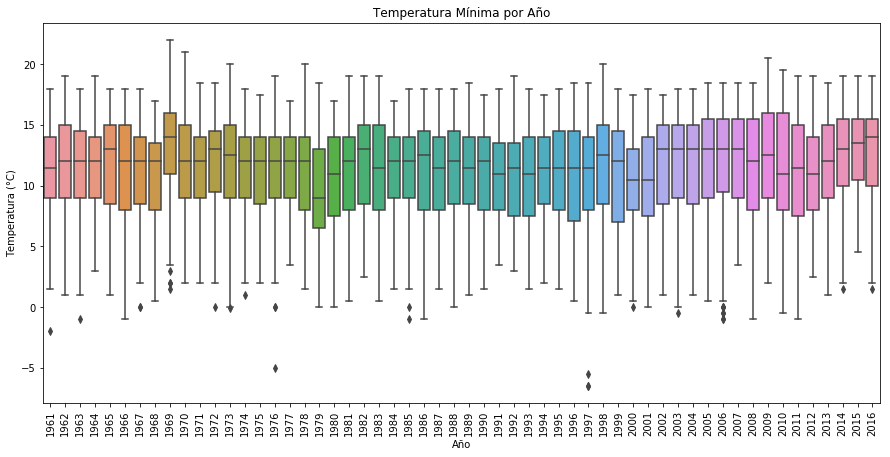
\includegraphics[scale = 0.5]{TminBoxY.png}
    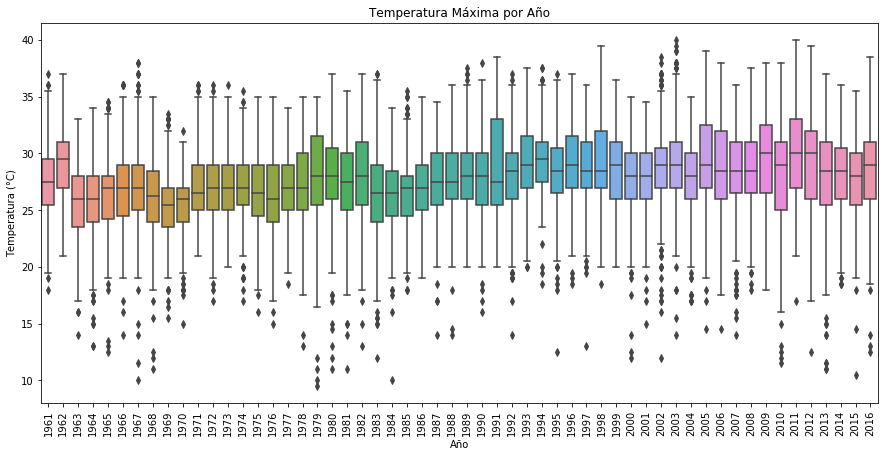
\includegraphics[scale = 0.5]{TmaxBoxY.png}
\end{center}
\section{Conclusión}
\noindent Se cumplió con el objetivo principal de la actividad, la cual era conocer la librería de Matplotlib en Python un poco por encima para encender un poco la curiosidad en nosotros sobre el análisis de datos con Python y seguir buscando, por ejemplo, otros tipos de gráficos.

Es una herramienta esencial en el análisis de datos ya que te da una visualización general, rápida y eficiente, porque tenemos que trabajar con miles de datos y esto te ayuda a resumir a grandes rasgos lo que te están diciendo los datos. Es muy bueno para responder a preguntas rápidas que se hacen, como cuáles meses fueron los más cálidos como hemos visto en la actividad pasada. También es una forma más intuitiva de visualizar los datos y no sólo con tablas. Además existen muchos tipos diferentes de gráficas para cada situación. 

\clearpage
\section{Bibliografía}
\begin{itemize}
    \item Gallery. (2019). Consultado: 15 de Febrero del 2019, de Matplotlib.org. Sitio web:
    
    https://matplotlib.org/gallery/index.html
    
    \item Matplotlib Tutorial: Python Plotting. (2017). Consultado: 15 de Febrero del 2019, de DataCamp. Sitio web: 
    
    https://www.datacamp.com/community/tutorials/matplotlib-tutorial-python
    
    \item What is Matplotlib?. (2017). Consultado: 18 de Febrero del 2019, de edureka!. Sitio web:
    
    https://www.edureka.co/blog/what-is-matplotlib/
    
    \item Boxplots. (2019). Consultado: 17 de Febrero del 2019, de Matplotlib.org. Sitio web:
    
    https://matplotlib.org/gallery/statistics/boxplot\_demo.html
    
    \item Representación gráfica de funciones y datos. (2018). Consultado: 18 de Febrero del 2019, de IAC. Sitio web: 
    
    http://www.iac.es/sieinvens/python-course/source/matplotlib.html

    \item Python, R, and Linux Tips. (2018). Consultado: 19 de Febrero del 2019, de CMD Line Tips. Sitio web: 
    
    http://cmdlinetips.com/2018/03/how-to-make-boxplots-in-python-with-pandas-and-seaborn/
    
    \item Boxplot placed on time axis. (2017). Consultado: 18 de Febrero del 2019, de stackoverflow. Sitio web:
    
    https://stackoverflow.com/questions/38576692/boxplot-placed-on-time-axis
    
    \item Matplotlib: Group boxplots. (2016). Consultado: 18 de Febrero del 2019, de stackoverflow. Sitio web:
    
    https://stackoverflow.com/questions/16592222/matplotlib-group-boxplots
    
    \item Agrupación de datos por fecha en pandas. (2018). Consultado: 15 de Febrero del 2019, de Analytics Lane. Sitio web:
    
    https://www.analyticslane.com/2018/07/06/agrupacion-de-datos-por-fecha-en-pandas/
    
    
    
\end{itemize}


\end{document}
